
\documentclass[sigconf]{acmart}

\usepackage{booktabs} % For formal tables
\usepackage{caption}
\usepackage{subfig}
\usepackage{url}
\usepackage{epstopdf}
%\usepackage{graphics,graphicx}
%\usepackage{cite}%
%\usepackage{epsfig}
\usepackage{array}
\usepackage{pifont}
\usepackage{multirow}
%\usepackage{fixltx2e}
\usepackage{amssymb}
\usepackage{footnote}
\usepackage{tablefootnote}
%\usepackage[utf8]{inputenc}
%\usepackage[TS1,T1]{fontenc}


%\usepackage[latin1]{inputenc}


% Copyright
%\setcopyright{none}
%\setcopyright{acmcopyright}
%\setcopyright{acmlicensed}

%\setcopyright{rightsretained}  % this was un-commented originally - SG
\setcopyright{iw3c2w3}
% added by KH as per https://www.overleaf.com/14253237rhxnsnkxskbb#/54980477/


%%%%%%%%%%%%%%%%%%%%%%%%%%%%
% DOI
\acmDOI{10.1145/3184558.3191623}

% ISBN
\acmISBN{978-1-4503-5640-4/18/04}

%Conference
\acmConference[WWW'18 Companion]{The 2018 Web Conference Companion}{April 23--27, 2018}{Lyon, France}
\acmBooktitle{WWW'18 Companion: The 2018 Web Conference Companion, April 23--27, 2018, Lyon, France}
\acmYear{2018}
\copyrightyear{2018}
\acmPrice{}
% \bookTitle{The 2018 Web Conference Companion, April 23--27, 2018, Lyon, France}
%%%%%%%%%%%%%%%%%%%%%%%%%%%


\usepackage{color}
\newcommand{\todo}[1]{\textcolor{red}{TODO: #1}}
\newcommand{\new}[1]{\textcolor{blue}{#1}}

\fancyhead{}

\begin{document}

\title{SAVITR: A System for Real-time Location Extraction from Microblogs during Emergencies}

\author{Ritam Dutt}
\affiliation{%
  \institution{Dept. of Computer Science and Engineering}
  \streetaddress{}
  \city{Indian Institute of Technology Kharagpur}
  \state{India}
  \postcode{721302}
}
\email{ritam@iitkgp.ac.in}

\author{Kaustubh Hiware}
\affiliation{%
  \institution{Dept. of Computer Science and Engineering}
  \streetaddress{}
  \city{Indian Institute of Technology Kharagpur}
  \state{India}
  \postcode{721302}
}
\email{hiwarekaustubh@iitkgp.ac.in}

\author{Avijit Ghosh}
\affiliation{%
  \institution{Dept. of Chemical and Financial Engineering}
  \streetaddress{}
  \city{Indian Institute of Technology Kharagpur}
  \state{India}
  \postcode{721302}
}
\email{avijitg22@iitkgp.ac.in}

\author{Rameshwar Bhaskaran}
\affiliation{%
  \institution{Dept. of Computer Science and Engineering}
  \streetaddress{}
  \city{Indian Institute of Technology Kharagpur}
  \state{India}
  \postcode{721302}
}
\email{rameshwar.cs@iitkgp.ac.in}

% The default list of authors is too long for headers}
\renewcommand{\shortauthors}{R. Dutt et al.}


\begin{abstract}
We present SAVITR, a system that leverages the information posted on the Twitter microblogging site to monitor and analyse emergency situations.
Given that only a very small percentage of microblogs are geo-tagged, it is essential for such a system to extract locations from the text of the microblogs.
We employ natural language processing techniques to infer the locations mentioned in the microblog text, in an unsupervised fashion and display it on a map-based interface. 
The system is designed for efficient performance, achieving an F-score of 0.81, and is approximately two orders of magnitude faster than other available tools for location extraction. 








\end{abstract}


%\if 0
%
% The code below should be generated by the tool at
% http://dl.acm.org/ccs.cfm
% Please copy and paste the code instead of the example below. 
%
 \begin{CCSXML}
<ccs2012>
<concept>
<concept_id>10002951.10003317</concept_id>
<concept_desc>Information systems~Information retrieval</concept_desc>
<concept_significance>500</concept_significance>
</concept>
</ccs2012>
\end{CCSXML}

\ccsdesc[500]{Information systems~Information retrieval}

%\fi

% We no longer use \terms command
%\terms{Theory}

\keywords{Emergencies, microblogs, location extraction, Geonames}


\maketitle



\section{Introduction}

Online social media sites, especially microblogging sites like Twitter and Weibo, have been shown to be very useful for gathering  situational information in real-time~\cite{social-media-emergency-survey,rudra-cikm-disaster}. 
Consequently, it is imperative to not only process the vast incoming data stream on a real-time basis, but also to extract relevant information  from the unstructured and noisy data accurately.

It is especially crucial to extract geographical locations from tweets (microblogs), since the locations help to associate the information available online with the physical locations.
This task is challenging since geo-tagged tweets are very sparse, especially in developing countries like
India, accounting for only 0.36\% of the total tweet traffic.
Hence it becomes necessary to extract locations from the text of the tweets.
%Additionally, geo-tags in tweets are not necessarily an
%accurate representation of the situation. Users are free to post about a remote incident from their current position.
This work proposes a novel and fast method of extracting locations from English tweets posted during emergency situations. 
The location is inferred from the tweet-text in an unsupervised fashion as opposed to using the geo-tagged field. 
%Our work addresses the two key research questions:
%\noindent \textbf{RQ1}: What is the performance of the location detection algorithm in terms of coverage and accuracy?
%\noindent \textbf{RQ2:} Is our method reliably deployable, i.e., is it able to capture an unexpected emergency scenario accurately? 

Note that several methodologies for extracting locations from tweets
have been proposed in literature; some of these are discussed in the next section. 
We compare the proposed methodology with several existing methodologies
in terms of coverage (Recall) and accuracy (Precision). 
Additionally, we also compared the speed of operation of different methods, which is crucial for real-time deployment of the methods. 
The proposed method achieves very competitive values of Recall and Precision with the baseline methods, and the highest F-score among all methods.
Importantly, the proposed methodology is several orders of magnitude faster than most of the prior methods, and is hence 
suitable for real-time deployment. 

We deploy the proposed methodology on a system available at \url{http://savitr.herokuapp.com}, which is described in a later section.

\section{Related Work}

We discuss some existing information systems for use during emergencies, and some prior methods for location extraction from microblogs.

\subsection{Systems for emergency informatics}

A few Information Systems have already been implemented in various countries for emergency informatics, and their efficacy has been demonstrated in a variety of situations. 
Previous work on real-time earthquake detection in Japan was deployed by~\cite{Sakaki} using Twitter users as social sensors. 
Simple systems like the Chennai Flood Map~\cite{Mapbox} have demonstrated the need and utility of Information Systems during the 2015 floods in the city of Chennai, India.
This system used a combination of crowdsourcing, open source mapping technologies and contributed to large-scale civic participation.

% It used a combination of crowdsourcing, open source mapping technologies and contributed to large-scale civic participation. 
Likewise, Ushahidi~\cite{Ushahidi} is a non-profit crisis-mapping software
company which utilises the concept of crowdsourcing for social
activism and public accountability. It enables local observers to submit reports using their mobile phones or the Internet, thereby creating a temporal and geospatial archive of an ongoing event. 
Ushahidi has been deployed in situations such as earthquakes in Haiti, Chile, forest fires in Italy and Russia.

% It has been developed by the Qatar Computing Research Institute in collaboration with United Nations Office for Coordination of Humanitarian Affairs (OCHA) and the UN International Children’s Fund (UNICEF).
%The potential of crowdsourcing can also be acknowledged from the success of AIDR \cite{aidr}, a platform designed for classifying crisis-related microblogs (tweets). It has been developed by the Qatar Computing Research Institute in collaboration with United Nations Office for Coordination of Humanitarian Affairs (OCHA) and the UN International Childrens Fund (UNICEF).

The system developed in the present work functions on the same basic principle as the aforementioned ones -- information extraction from crowdsourced data. 
However, unlike Mapbox~\cite{Mapbox} and Ushahidi~\cite{Ushahidi}, it is not necessary for the users to explicitly specify the location. Rather, we infer it from the tweet text, without any prior manual labeling. 


\subsection{Location Inferencing methods}

Location inferencing is a specific variety of Named Entity Recognition (NER), whereby only the entities corresponding to valid geographical locations are extracted. 
There have been seminal works regarding location extraction from microblog text, inferring the location of a user from the user's set of posted tweets and even predicting the probable location of a tweet by training on previous tweets having valid geo-tagged fields.
Publicly available tools like Stanford NER \cite{StanfordNER}, TwitterNLP \cite{TwitterNLP1}, OpenNLP \cite{OpenNLP} and Google Cloud\footnote{https://cloud.google.com/natural-language/}, are also available for tasks such as location extraction from text.

We focus our work only on extracting the locations from the tweet text, since we have observed that 
(i)~a very small fraction of tweets are geo-tagged~\footnote{Note that in a geo-tagged tweet, the location is explicitly provided by the user as a separate field, regardless of whether it is present in the text}, and 
(ii)~even for geo-tagged tweets, a tweet's geo-tagged location is not always a valid representative of the incident mentioned in the tweet text. 
For instance, the tweet ``{\it Will discuss on \@TimesNow at 8.30 am today regarding Dengue Fever in Tamil Nadu.}'' clearly refers to Tamil Nadu, 
but the geo-tagged location is New Delhi (from where the tweet was posted). 



We give an overview of the different types of methodologies used
in location extraction systems.
Prior state-of-the-art methods have performed common preprocessing steps like noun-phrase extraction and phrase matching~\cite{Malmasi}, or regex matching~\cite{twitie} before employing some of the following techniques for location extraction. 
\begin{itemize}
\item{Gazetteer lookup:}
Gazetteer based search and n-gram based matching have been employed by  \cite{Malmasi}, \cite{middleton} , \cite{gelernter}. Usually some publicly available gazetteers like GeoNames or OpenStreetMap are used.

\item{Handcrafted rules} were employed in \cite{Malmasi} and \cite{gelernter}

\item{Supervised methods:}
Well-known supervised models used in this current context are:
\begin{enumerate}
\item{Models based on Conditional Random Fields (CRF)} such as the Stanford NER parser which was employed by \cite{gelernter} and \cite{Malmasi}. While \cite{gelernter} trained the model on tweet texts, \cite{Malmasi} used the parser without training.
\item{Maximum entropy based models} such as the OpenNLP was deployed by \cite{lingad} without training and it infers location using ME.
\end{enumerate}

\item{Semi-supervised methods:}
The work~\cite{ji2016joint} used semi-supervised methods such as beam-search and structured perceptrons to label sequences and linked them with corresponding Foursquare location entities. 

\end{itemize}




%Consequently the unsupervised algorithm assures that our system is capable of integrating news from different sources. Moreover, unlike other systems which are used during crisis analysis, ours intend to detect the onset of some calamity, by analysing past trends. 


%%%%%%%%%%%%%%%%%%%%%%%%%%%%%%%%%%%%%%%%%%%%%%%%%%%%%%%%
\section{Extracting locations from microblogs}

We now describe the proposed methodology for inferring locations from tweet text. The methodology involves the following tasks.

\subsection{Hashtag Segmentation}

Hashtags are a relevant source of information in Twitter. Especially for tweets posted during emergency situations, hashtags often contain location names embedded in them, e.g., \#NepalQuake, \#GujaratFloods, \#puertorico, \#HoustonStrong, \#MumbaiRains. 
In fact, it was observed that there are as many as 21 valid  locations among the 100 most frequent hashtags posted during some recent emergency events related to floods, earthquakes and rain.
However, due to the peculiar style of coining hashtags, it becomes imperative to break them into meaningful words. 
Similar to~\cite{Malmasi} and~\cite{DBLP:journals/corr/abs-1708-03105}, we adopt a statistical word segmentation based algorithm~\cite{Peter} to break a hashtag into distinct words, and extract locations from the distinct words. 
We also retain the original hashtag, to ensure we do not lose out on meaningful remote locations simply because they are uncommon. 
 
%An example of a correct and incorrect hashtag segmentation is demonstrated here. 

%Correct hashtag segmentation example:\\
%\textit{\#GujaratFloods  When the floods devastated Gujarat in 2016 and 2017 our Khalsa Aid India based volunteers were there} \\
%\#GujaratFloods $\rightarrow$ gujarat, floods

%Incorrect hashtag segmentation example:\\
%\textit{Weve dispatched off equipment to \#Kabale and \#Kisiizi [hospital] as an emergency intervention following recent devastations}. 
%Here \#Kisiizi is broken down to kissi and zi, despite Kisiizi hospital being a verifiable place in Uganda. 

We have observed that hashtag segmentation has some unforeseen outcomes. While trying to optimize recall from a tweet, it hampers precision, especially when the segmented words corresponds to actual locations. 
For example `\#Bengaluru' (a place in India) is broken down into `bengal' and `uru', which are two other places in India. 
Likewise,`\#Kisiizi hospital', a hospital in Uganda, in the tweet "\textit{We've dispatched off equipment to \#Kabale and \#Kisiizi hospital as an emergency intervention following recent devastations}", is incorrectly segmented into `kissi' and `zi', none of which are location names.
In spite of these limitations of hashtag segmentation, we still carry out this step since we seek to extract all possible location names, including those embedded within hashtags. 


\subsection{Tweet Preprocessing}

We have employed common pre-processing techniques on the tweet text to remove URLs, mentions, stray characters like brackets, 'RT', \#, \&, ellipses and specific Unicode characters corresponding to emojis as observed in Figure \ref{fig:Flowchart}.
We also segmented CamelCase words and joint alphanumeric terms like `Chennai2015' into distinct terms (`Chennai' and `2015').
We did {\it not} perform case-folding on the text since we wanted to detect proper nouns. Likewise, we also abstained from stemming since location names might get altered and cannot be detected using the gazetteer.


\subsection{Disambiguating Proper Nouns from Parse Trees}

Since most location names are likely to be proper nouns, we use a heuristic to determine whether a proper noun is a location. 
We first apply a Parts-of-Speech (POS) tagger to yield POS tags.
%We present here our heuristic for ascertaining a proper noun as a location. The tweet text obtained after pre-processing was parsed to yield Parts of Speech (POS) tags. 
There are several POS taggers publicly available, which could be applied, such as SPaCy\footnote{https://spacy.io/}, the Twitter-specific 
CMU TweeboParser\footnote{http://www.cs.cmu.edu/~ark/TweetNLP/}, and so on.
We employ the POS Tagger of SPaCy, in preference to the CMU TweeboParser, due to the heavy processing time of the latter. The TweeboParser was 1000 times slower as opposed to SpaCy. 
We considered the speed to be a viable trade-off for accuracy since we want the method to be deployed on a real-time basis and we observed the processing time would be a bottleneck in this regard.

Let $T_{i}$ denote the POS tag of the $i^{th}$ word $w_i$ of the tweet. If $T_{i}$ corresponds to a proper noun, we keep on appending words that succeed $w_i$, provided they are also proper nouns, or adjectives or delimiters (conjunctions (`and', `or') or punctuations (`;', `)' ). 
We have developed a list of common suffixes of location names (explained below). 
If $w_i$ is followed by a noun in this suffix list, we consider it to be a viable location. Acknowledging the fact that Out of Vocabulary (OOV) words are common in Twitter, we also consider those words which have a high Jaro-Winkler similarity with the words in the suffix list.
We also check the word immediately preceding $w_i$, to see if it is a preposition that usually precedes a place or location, such as `at', `in', `from', `to', `near', etc, or directions like north, eastern etc.  
We then split the stream of words obtained via the delimiters.
Thus, we attempt to infer from the text proper nouns which conform to locations from their syntactic structure. 

We illustrate the working of this procedure using the processed tweet text `\textit{18 doctors on 18 motorcycles rode to 132 flood-hit villages in Bainsa division of Purnia district in Bihar} also depicted in the flowchart in 
Figure~\ref{fig:Flowchart}. 
The algorithm identifies 'Bainsa', 'Purnia' and 'Bihar' as proper nouns. Since `Purnia' is followed by the word `district', the phrase `Purnia district' is identified as a location. However, `Bainsa' and `Bihar' are also detected as viable locations because they were treated as prepositional objects with respect to the preposition `in'. 



\subsection{Regex matches}

As mentioned in the previous section, we have compiled a suffix list 
%and prefix list that usually append or prepend a location respectively, some being mentioned in Table ~\ref{tab:Example list}
containing words that usually come after a location name. 
The suffix list comprises different naming conventions for
landforms\footnote{https://en.wikipedia.org/wiki/List\_of\_landforms}, 
roads\footnote{https://wiki.waze.com/wiki/India/Editing/Roads} \footnote{http://www.haringey.gov.uk}, 
buildings\footnote{https://en.wikipedia.org/wiki/List\_of\_building\_types} and towns 
In a similar fashion, we have also compiled a prefix list, which specifies the direction that prepend a location, like Southern California, West Bengal.
A part of the suffix and prefix list is shown in Table~\ref{tab:Example list}.

We identify the prefix and suffix elements from the tweet text and treat the words that succeed or precede it as viable locations.
We perform this additional task of regex similarity to account for cases when the tweet is posted in lowercase, making it difficult to detect and disambiguate proper nouns.
Using the suffix list enables us 
to detect places like `Vinayak hospital' and `Gujranwala town' from the tweet ``\textit{Urgent B+ group platelets suffering from dengue,Ankit Arora  At Vinayak hospital, Gujranwala town,delhi}''.

\begin{table}[tb]
% Center the table
\centering
	% Title of the table
	\begin{tabular}{|c|c|}
	% To create a horizontal line, type \hline
	\hline
	% To end a column type &
	% For a linebreak type \\
	Type & Common Examples\\ \hline
	
	Landforms & doab, lake, steam, river, island, valley, mountain, hill \\
	Roads & street, st, boulevard, junction, lane, rd, avenue, bridge\\
	Buildings & hospital, school, shrine, cinema,villa, temple, mosque,  \\
	Towns & city, district, village, gram, place,town, nagar,  \\
	Directions & south, eastern, NW, SE, west, western, north east,\\
	\hline
	Diseases & dengue, ebola, cholera, zika, malaria, chikungunya  \\
	Disasters & earthquake, floods, drought, tsunami, landslide, rains\\
	
	\hline
	\end{tabular}
  	\caption{Examples of suffixes and emergency-related words}
	\label{tab:Example list}
\vspace*{-5mm}
\end{table}

%The prefix list specifies the direction that comes before a position, like Southern California, West Bengal. We extract phrases of length 2 to 3 that are followed by the suffixes and phrases of length 2 to 3 that follow the prefixes, provided none of the words in the phrase occur infrequently.
\begin{figure*}[tb]
	% Center the figure.
	\centering
		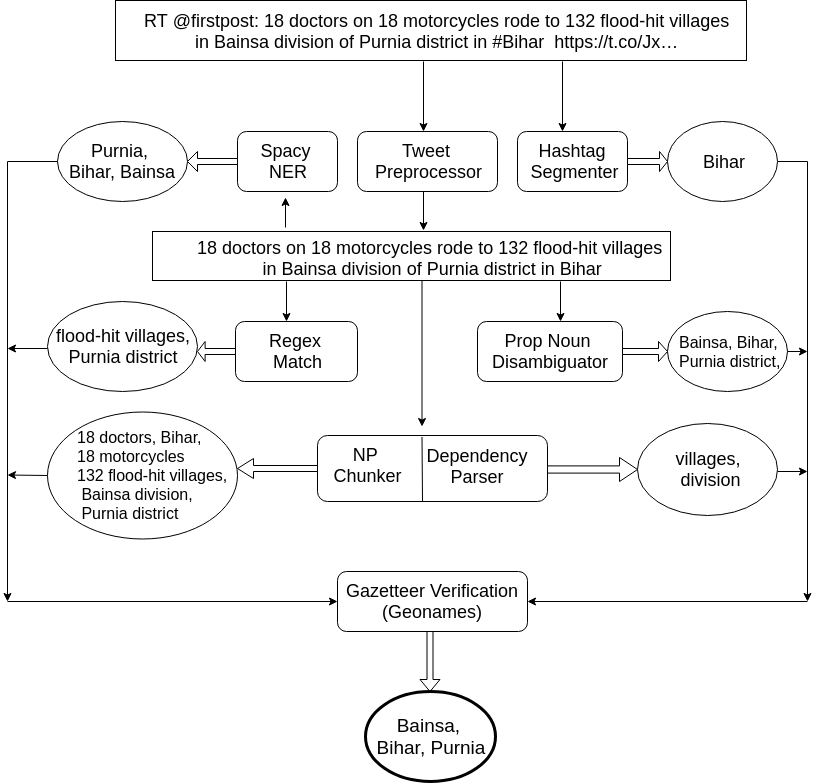
\includegraphics[height=10cm, width=0.6\textwidth]{Flowchart}
		% Create a subtitle for the figure.
		\caption{Flowchart depicting the functioning of our algorithm on a sample tweet ``{\it RT \@firstpost: 18 doctors on 18 motorcycles rode to 132 flood-hit villages in Bainsa division of Purnia district in \#Bihar  https://t.co}''.}
		\label{fig:Flowchart}
\vspace*{-5mm}
\end{figure*}





\subsection{Dependency Parsing of Emergency words}

So far, the  methodology aims at improving the precision, by considering specific norms or patterns by which locations are usually identified. This step is meant to improve recall by capturing those locations which do not follow the common patterns listed above.

Taking into consideration that our objective is to monitor emergency scenarios, we identify a comprehensive set of words corresponding to 
epidemic disasters\footnote{https://en.wikipedia.org/wiki/List\_of\_epidemics} and natural disasters\footnote{https://en.wikipedia.org/wiki/Lists\_of\_disasters}, some of which are shown in Table ~\ref{tab:Example list}.
We identify the list of emergency words in the tweet text and consider words, namely proper nouns, nouns and adjectives, which are {\it at a short distance of 3-4 from the emergency word} in the dependency graph obtained for the tweet text.
The distance metric refers to the number of links connecting the words in the dependency graph of the tweet text. A short dependency implies the word is more intimately affected by the emergency word.
We had taken randomly 100 tweets which had 153 locations identifiable by manual annotation, out of which 139 were correctly identified. The average distance between the emergency word and the identifiable locations via the dependency graph was found to be $3.942$ while the orthographic distance (the number of words between the emergency and and target word ) was $5.111$.

As an example, Figure~\ref{fig:dependency_graph} shows the dependency graph for the tweet ``{\it Mumbai lost its mudflats and wetlands, now floods with every monsoon.}''.
We see that the distance between Mumbai and floods in the dependency graph of the tweet is 2, whereas the actual distance between the words in the text is 7. Hence we can identify Mumbai as a proper location via dependency parsing.

Thereafter, we also extract the noun phrases from the dependency graph similar to ~\cite{Malmasi}. These noun phrases can represent potential locations as illustrated in the \ref{fig:Flowchart}, wherein the NP (Noun Phrase) Chunker gave viable locations like `Purnia district', `Bainsa division', besides redundant information like `132 flood-hit villages'. 
Finally, for sake of completeness, we use an NER tagger in a fashion similar 
to~\cite{Malmasi,lingad,gelernter}. 
We have leveraged the NER Tagger provided by SpaCy as opposed to the more commonly available NER tools like Stanford NER~\cite{StanfordNER}, 
Twitter NLP~\cite{TwitterNLP1}, 
Open NLP~\cite{OpenNLP}, due to the faster execution time of the former as observed in Table \ref{tab:Evaluation table}.


\begin{figure}[tb]
	% Center the figure.
	\centering
		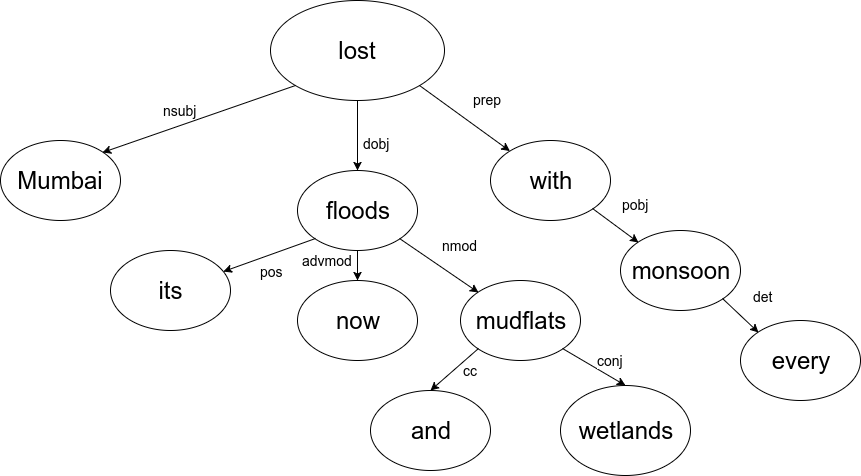
\includegraphics[scale=0.27]{dependency_graph}
		% Create a subtitle for the figure.
		\caption{Dependency graph for a sample tweet ``{\it Mumbai lost its mudflats and wetlands, now floods with every monsoon.}''.}
		\label{fig:dependency_graph}
\vspace*{-5mm}
\end{figure}


\subsection{Gazetteer Verification}

The list of phrases and locations extracted by the above methods are then verified using a gazetteer, to retain only those words that correspond to real-world locations. As evident from Figure~\ref{fig:Flowchart}, the gazetteer verification step is essential to filter out redundant noun phrases and nouns obtained via dependency parsing and regex matches, such as `18 doctors', `flood-hit villages', `division', etc.
For our system, the gazetteers also returns the geo-spatial coordinates to enable plotting the location on a map. The gazetteer choice depends upon the granularity and precision of our location and also on the performance speed. There is a trade-off for finer accuracy against performance which we illustrate in the later sections.



%


\section{Comparative evaluation of the location inference}

In this section, we describe the evaluation of the proposed methodology,
and compare it with several baseline methods.
We start by describing the dataset and some design choices made by us.

\subsection{Dataset}

We used the Twitter Streaming API\footnote{https://developer.twitter.com/en/docs}, to collect tweets from 12$^{th}$ September, 2017 to 13$^{th}$ October, 2017, and filtered those tweets that contained either of the two words 'dengue' or 'flood'. 
This step produced a dataset of 317,567 tweets collected over a period of 31 days. The tweets were preprocessed to remove duplicates and also tweets written in non-English languages. 
This filtering resulted in 239,276 distinct tweets. 
%Out of these, only 0.36\% were geo-tagged -- this small percentage motivates the need for location inference from the tweet text. 
%These were further segregated into tagged and untagged based on the presence of a valid location.

\subsection{Gazetteer employed}

In this work, we currently focus on collecting and displaying tweets within the bounding box of the country of India. 
Thus, we need some lexicon / gazetteer to disambiguate whether a place is located inside India and what its geographical coordinates are. 
To that end, we scraped the data publicly available from Geonames\footnote{http://www.geonames.org/} and created a dictionary corresponding to different locations within India. 
The dictionary has the information of $449,973$ locations within India. 
However, some places mentioned in this dictionary have high orthographic similarity with common English nouns. For example, we find that 
the word `song' is a place located in Sikkim (within India), whose coordinates are \(27.24641 'N, 88.50622 'E\). Moreover, Geonames does {\it not} contain fine-grained information of addresses such as roads and buildings. 

Consequently, we explored another gazetteer -- 
the Open Street Map gazetteer\footnote{http://geocoder.readthedocs.io/providers/OpenStreetMap.html} 
which has a comprehensive list of all possibles addresses for India. However, the sheer volume of the data -- $\approx 530$ times larger than Geonames -- hampers performance in a real-time setting. 
Also, API calls take considerable time as opposed to querying the downloaded dump of the Geonames Gazetteer\footnote{http://download.geofabrik.de/asia/india.html}.

Thus the choice of the gazetteer is governed by a trade-off
between recall and efficiency. 
We report performances using both gazetteers in this paper. Hence we consider two variants of the proposed methodology:
\begin{itemize}
\item GeoLoc - Our proposed methodology using Geonames as the gazetteer. 
\item OSMLoc - Our proposed methodology using Open Street Maps as the gazetteer. 
\end{itemize}



\subsection{Baseline methodologies}

We compared the proposed approach of our algorithm with several baseline methodologies which are enlisted below: 
\begin{itemize}
\item UniLoc- Take all unigrams in the processed tweet text and infer if any of those correspond to a possible location (by referring to a gazetteer). 
\item BiLoc- Similar to UniLoc, except we consider both unigrams and bigrams in the tweet text.
\item StanfordNER - Employs the NER of coreNLP parser~\cite{StanfordNER}. 
\item TwitterNLP - Employ the NER of Twitter NLP parser developed by Ritter et al.~\cite{TwitterNLP1}
\item GoogleCloud - Use the Google Cloud Natural Language Platform to infer locations.\footnote{https://cloud.google.com/natural-language/}
\item SpaCyNER - Use the trained SpaCy NER tagger. 
\end{itemize}	
For all the baseline methods, the potential locations are checked using the GeoNames gazetteer. 


\subsection{Evaluation Measures}

Given a tweet text, we wish to infer all possible locations contained in the tweet. Thus we should prefer a method which has higher recall. However, since we also aim to plot the location obtained from the tweet, the precision of our extracted locations also matters. Hence we apply the following measures.
\begin{equation}
Precision =\frac{\left | \mbox{Correct Locations} \bigcap \mbox{Retrieved Locations}  \right |}{ \mbox{Retrieved Locations}}
\end{equation}
\begin{equation}
Recall =\frac{\left | \mbox{Correct Locations} \bigcap \mbox{Retrieved Locations}  \right |}{ \mbox{Correct Locations}}
\end{equation}
%\begin{equation}
%FScore = \frac{2 \times Precision \times Recall}{Precision+Recall}
%\end{equation}
where `Correct locations' is the set of locations actually mentioned in a tweet, as found by human annotators, and
`Retrieved locations' is the set of locations inferred by a certain methodology from the same tweet.
To get an idea of both precision and recall, we use F-score which is the harmonic mean of precision and recall.

Moreover, since we wish to deploy the system on a real-time basis, the {\it evaluation time} taken by a method is also a justifiable metric.



\subsection{Evaluation results}

We randomly selected 1,000 tweets from the collected set of tweets (as described earlier), and asked human annotators to identify those tweets which contain some location names.
The annotators identified a set of 99 tweets that contained at least one location name, all of which were located within India's geographical boundaries. Hence the comparative evaluation is carried out over this set of 99 tweets.
Table~\ref{tab:Evaluation table} compares the performances of the baseline methods and the proposed method.
The last column shows the total time in seconds needed to process the $99$ tweets that we are using for evaluation.

%The seven methods were tested on a set of 101 tweets obtained at random from the entire corpus of the tweets collected during this time frame. All the tweets have at least one location and all the locations are within India.

\begin{table}[tb]
	% Center the table
	\centering
		% Title of the table
		\begin{tabular}{|c|c|c|c|r|}
			% To create a horizontal line, type \hline
			\hline
			% To end a column type &
			% For a linebreak type \\
			Method&	Precision&	Recall&	F-score&	Timing (in s)\\
			\hline
			UNILoc&	0.3848&	0.7852&	0.5165&	0.0553\\
			BILoc&	0.4025&	0.8590&	0.5482&	0.0624\\
			StanfordNER& 0.8103&	0.6322&	0.6988&	175.0124\\
			TwitterNLP&	0.6356&	0.5474&	0.5882&	28.0001\\
			GoogleCloud &	0.6321&	0.5339&	0.5789&	NA\\
            SpaCyNER & \textbf{0.9883}& 0.5555&0.7113 &1.0891\\
            \hline
			GeoLoc &	0.7987&	0.8300&\textbf{0.8141}&	1.1901\\
			OSMLoc & 0.3383& \textbf{0.8888}&0.4901 &711.5817\\
            GeoLocNoNER& 0.7987&	0.7987&0.7987&	1.1687\\

			\hline
			
			\hline
		\end{tabular}
		\caption{Evaluation Performance of the baseline methods and the proposed methods (two variants, one using GeoNames gazetteer, and the other using Open Street Maps gazetteer).}
		\label{tab:Evaluation table}
        \vspace*{-5mm}
\end{table}


We observe that GeoLoc performs the best in terms of F1 score as compared to all other methods. It also scores high on precision, ranking only third to StanfordNER and SpaCyNER. The high precision of SpaCyNer is counterbalanced by its poor recall due to which it was hardly able to detect remote places.
For instance, for the tweet {\it `Urgent B+ blood needed for a crit dengue patient at May Hosp. , Mohali,(Chandigarh)'}, SpaCyNer fails to detect locations like `Mohali' from the tweet.  
However, `Mohali' is detected by our GeoLoc algorithm.

The slight decrease in precision is attributed to some common words like `song', `monsoon', `parole' being chosen as potential locations due to incorrect hashtag segmentation, and then the gazetter tagging these words as locations, since these are also names of certain places in India. 
%These are actual places located within India's geographical boundaries and hence Geonames tags them as valid locations. These names arise due to incorrect hashtag segmentation \footnote{504 kids died in Govt-aided hospital in \#Bengaluru . Many died in Kolar. But there’ s no end to shamelessness of...} or due to close proximity of the word to event related keywords \footnote{Mumbai lost its mudflats and wetlands , now floods with every monsoon . Cities need ecology AND restoration to}. The former segments Bengaluru into bengal and uru, both valid and common names in India, the latter misclassifies monsoon due to its short dependency path from floods.

It can also be seen that, the proposed method using GeoNames gazetteer is much faster than the other methods which achieve comparable performance (e.g., StanfordNER). 
We also note the performance of our proposed algorithm in the absence of any NER tool, denoted by GeoLocNoNER in the Table \ref{tab:Evaluation table}. It is observed that our proposed methodology performs better than the pre-existing ones and suffer only a slight decrease in recall (3.7\%) as compared to GeoLoc. This validates the claim that our proposed methodology is not solely dependent on the accuracy of the NER tool employed. 

\vspace{3mm}
\noindent {\bf Choice of gazetteer:}
As stated earlier, the Geonames gazetteer lacks information of a granular level. Consequently specific places pertaining to hospitals and streets are often not recognized as valid locations. This hampers the recall of the system, e.g., the proposed methodology was unable to detect `star hospital' in the tweet ``{\it We need O-ve blood grup for 8 years boy suffering with dengue in star hospital in karimnagar , please Contact}.''

Open Street Map (OSM) is able to detect such specific locations and thus exhibits the highest recall amongst all other methods. However, using OSM has the side-effect of classifying many simple noun phrases as valid locations. For instance, 
`silicon city' is detected as a location in the tweet ``{\it @rajeev\_mp  seems its time to rename Bangalore as Floods city I/O silicon city.}'', since `silicon city' is judged a shortening for the entry `Concorde Silicon Valley, Electronics City Phase 1, Vittasandra, Bangalore'. 
As a result of such errors, the method using OSM has the lowest precision score amongst all the methods. 


\vspace{3mm}
\noindent {\bf Performance over the entire dataset:}
%We also demonstrate the efficiency of our algorithm in terms of coverage, which we define as the fraction of tweets which our algorithm has been able with a correct location field. 
From the entire set of 239,276 distinct tweets, only 
3,493 were geo-tagged, out of which 869 were from India (which corresponds to a minute $0.36\%$ of the entire dataset). 
The number of tweets which were successfully tagged from the entire dataset, using our proposed technique and Geonames was 68,793, which corresponds to approximately $26.15\%$. 
Hence the coverage increased drastically. 
The method could identify niche and remote places in India, like `Ghatkopar', `Guntur', `Pipra village' and `Kharagpur', besides metropolitan cities like `Delhi', `Kolkata' and `Mumbai'. 



%%%%%%%%%%%%%%%%%%%%%%%%%5
\if 0

\begin{table}[!hbt]
	% Center the table
	\begin{center}
		% Title of the table
		\caption{Coverage of tweets}
		\label{tab:Kerala}
		\begin{tabular}{|c|c|c|}
			% To create a horizontal line, type \hline
			\hline
			% To end a column type &
			% For a linebreak type \\
		{\footnotesize Tweet Text}&{\footnotesize TagLoc}& {\footnotesize GeoLoc} \\\hline
			{\footnotesize Numerous death in Kerala from Dengue,  Chicken guinea,}&{\footnotesize New Delhi}& {\footnotesize Kerala}\\
		{\footnotesize Malaria @cpimspeak pushed Kerala into a money order } & &\\\hline
			{\footnotesize @Bhayankur Hmmm - not rosy in Kerala either ...} & {\footnotesize New Delhi}& {\footnotesize Kerala}\\\hline
{\footnotesize Dengue : 5 worst affected states. Scandinavian } &{\footnotesize Bengaluru}& {\footnotesize Kerala}\\
			{\footnotesize level HDI state Kerala tops the list ... }& & \\\hline
			
			{\footnotesize 45\% of Dengue cases and nearly half the Dengue related }&{\footnotesize Bengaluru}&{\footnotesize Kerala,}\\
			{\footnotesize deaths in India from Kerala. Too much filth or related to}&& {\footnotesize India} \\\hline
			{\footnotesize @Rameshnair101 @CNNnews18 Dengue cases reported: },&{\footnotesize Kerala}&{\footnotesize Kerala,}\\
			 {\footnotesize UP 302 Kerala 16530 .death due to dengue: UP 17, Kerala 28}& &{\footnotesize UP} \\		
			\hline
			
			\hline
		\end{tabular}
	\end{center}
\end{table}

\fi
%%%%%%%%%%%%%%%%%%%%%%%%


\begin{figure}[tb]
	% Center the figure.
	\centering
		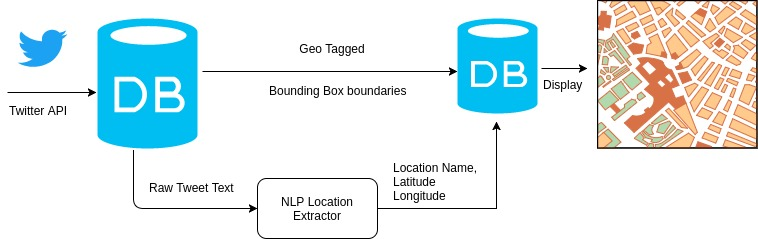
\includegraphics[scale=0.3]{system_arch}
		% Create a subtitle for the figure.
		\caption{System architecture of the SAVITR system}
		\label{fig:system_arch}
\end{figure}

\begin{figure}[tb]
	% Center the figure.
	\centering
		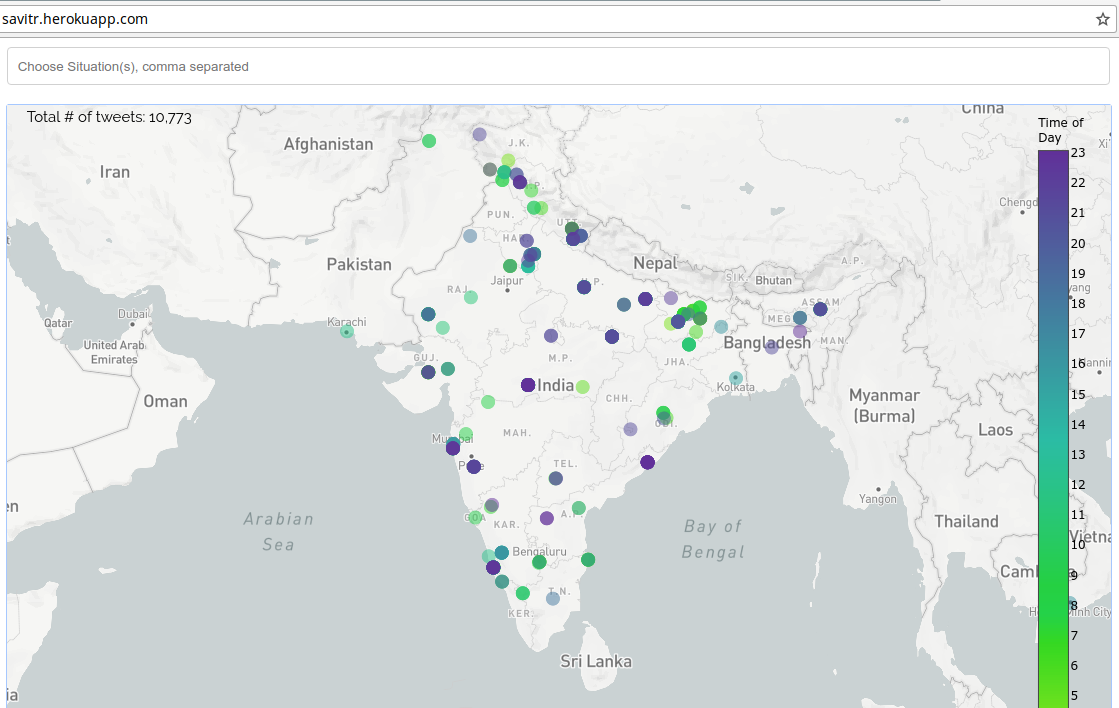
\includegraphics[scale=0.23]{map_general}
		% Create a subtitle for the figure.
		\caption{Snapshot of the SAVITR system: Tweets visualised on India's map}
		\label{fig:map_general}
	\vspace*{-5mm}
\end{figure}


\section{SAVITR: Deploying the location inference method}

\noindent We have deployed the proposed techniques (using GeoNames) on a system named SAVITR, which is live at \url{http://savitr.herokuapp.com}.
The software architecture of Savitr is presented in Figure~\ref{fig:system_arch}. 
Since the amount of data to be displayed is massive, we had to implement certain design considerations so that the information displayed is both compact and visually enriching, while at the same time scalable. 
The system was built using the Dash framework by Plotly~\cite{Plotly}. For our visualization purpose, we settled on a mapbox Map at the heart of the UI, with various controls, as described below. A snapshot
of the system is shown in Figure~\ref{fig:map_general}.
\begin{itemize}

\item A search bar at the top of the page. Whenever a term is entered into the search bar, the map refreshes and shows tweets pertaining to that query term. It also supports multiple search queries like "Dengue, Malaria".

\item The tweets on the map are color coded according to the time of the day. Tweets posted in the night are darker.

\item A date-picker -- if one wishes to visualize tweets posted during a particular time duration, this provides fine grained date selection, both at the month and date level.

\item A Histogram -- this shows the number of relevant (tagged) tweets posted per day.

\item Untagged tweets -- Finally, at the bottom of the page we display the tweets for which location could not be inferred (and hence they could not be shown on the map).
\end{itemize}

We report the performance of the system during the massive dengue outbreak that plagued India in the fall of 2017.\footnote{https://www.telegraphindia.com/india/dengue-spurt-in-south-182846} 
The state of Kerala was severely affected by the outbreak. 
%The report, published on 2$^{nd}$ November mentions the plight of the Southern States in the wake of dengue, some of the affected ones being Kerala and Tamil Nadu. We highlight the findings from our data in this aspect.
During this period, as many as $2204$ tweets mentioning Kerala were identified by the system, which is far higher than the average rate at which other locations were detected. 
Additionally, out of the $2204$ tweets containing the location `Kerala',
$1960$ ($88.92\%$) also contained the term `dengue' which is included in the list of disaster terms compiled by us (see Table~\ref{tab:Example list}).
These statistics demonstrate how the SAVITR system can be used as an `Early warning system' to flag any upcoming emergency situation.


Though the SAVITR system presently infers locations within India, it can be easily extended to infer locations within other countries, and the whole world in general. 
%The unnatural reference to these names as opposed to other metropolitan areas like Bangalore or Kolkata is proof that people are referring to these places more. This is evident as we observe the following statistics about Kerala. There were 2204 tweets about Kerala out of which 1960 tweets contain the term dengue. This amounts to a 88.92\% overlap.

%However most of the data is inferred  from the tweets having Kerala mentioned in their texts. We see some examples of geo-tagged tweets below which talk about Kerala but are posted from other parts of India. This paints an inaccurate description of the situaion. 




\section{Discussion}

A natural quest is to extend the scope of the system, e.g., to non-English tweets and to the whole world (instead of just India). 
To this end, we have observed several challenges that remains to be solved, some of which we enumerate in this section.

\subsection{Handling non-English tweets}

The methodology currently focuses on inferring locations from English tweets. However, the techniques in this paper leverage simple syntactic and semantic techniques and hence can be extended to other languages, like German and Hindi, provided the requisite tools (POS Tagger, dependency parser, lexicon) are available. We only need to craft the rules such as disambiguating proper nouns, in a manner which conforms with the grammatical structure.
However, the more challenging issue lies in extracting locations from code-mixed and code-borrowed tweets. A simple, crude technique would involve identifying the different languages from the tweet text, transliteration into English, and thereafter applying the algorithm as described in the paper. However whether this task can be accomplished on a real-time basis with decent accuracy remains unresolved.

\subsection{Identifying locations globally}

The system currently implemented focuses only on locations within the geographical boundaries of the country of India. 
We have experimented with different gazetteers at varying degrees of granularity and observed that a comprehensive/extensive gazetteer is able to capture finer-grained locations at the expense of greater misclassification. 
Thus, in order to infer locations on a global scale, we require a location disambiguation algorithm to distinguish between two distinct locations sharing the same name. For instance, the location `Kota' in the tweets "\textit{3 out of 6 members of my family had dengue last week in Kota, Rajasthan.}" and "\textit{Floods in Kota Belud cuts off access to 8 villages}" refer to a place in Rajasthan, India and another place in Malaysia respectively.

Any location disambiguation technique would need to rely on social cues, such as user-name of the person who posted the tweet, or the geo-tagged location of the tweet/user, in addition to the text. 
The short length of the tweet text might not be capable of providing sufficient context. However, in case of a global calamity, people all over the world express their opinion/ sympathy, which exacerbates the challenge of discerning the location of a text from the user name itself.

Likewise for some geo-tagged tweets, it is observed that a tweet can be posted from a different place as compared to the locations mentioned in the text. 
A common phenomenon is that a tweet posted from a metropolitan city (e.g., New Delhi) contains some information about a suburb. How to deal with such 
tweets is application-specific.

\subsection{System improvements}
Specific changes need to incorporated into the system as well if we intend to deploy it on a global scale. 
The massive information overload would deem it infeasible to display both tagged and untagged tweets on an individual basis. This necessitates implementing an automated summarization technique to capture and display summaries on the system. 
In the event of an epidemic, it is essential to classify tweets into different medical concepts like treatment, symptoms, transmission, death reports etc, which are important to different stakeholders. The system can be extended to display such crucial information on the map using different color codes. 


\section{Conclusion}

We proposed a methodology for real-time inference of locations from tweet text, and deployed the methodology in a system (SAVITR). The proposed methodology performs better than many prior methods, and is much more suitable for real-time deployment.
We also discussed the challenges that need to be solved for extending the scope of the system. 






\section*{Acknowledgements} 
The authors thank Dr. Saptarshi Ghosh, Department of Computer Science and Engineering, IIT Kharagpur, for mentorship and guidance throughout the project. 
The authors acknowledge the annotators (Sohan Patro and others) who helped in evaluation of the methodologies, and useful discussions with Nishant Nikhil in the early stage of the project. 
The authors also thank the anonymous reviewers whose comments helped to improve the paper.
The work is partially supported by Microsoft Research India, and part of the work was done at the 2017 MSR India Summer Workshop on Artificial Social Intelligence.


\bibliographystyle{ACM-Reference-Format}
\bibliography{twitter_references,reference} 

\end{document}

